\section{Analysis}
\begin{figure}[H]
	\centering
	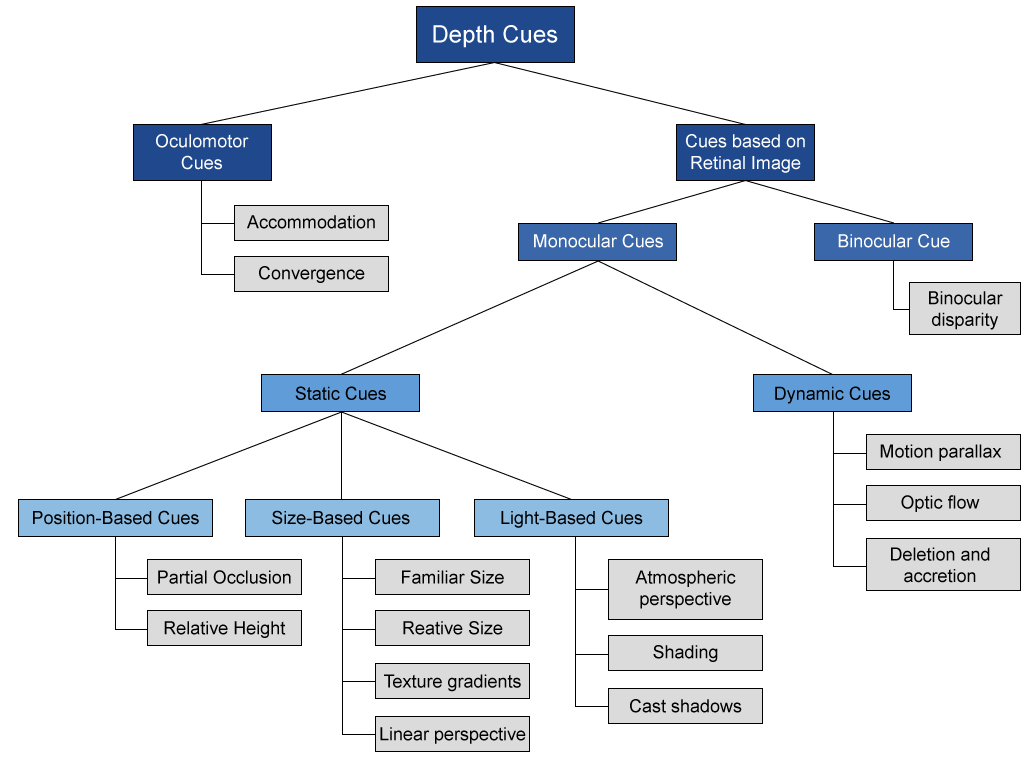
\includegraphics[width=1\linewidth]{figure/Analysis/depthCues.png}
	\caption{Model displaying the various depth cues. This model is a reconstruction of the model in the \textit{Sensation and perception} book\citep[p.~195]{sensationPerception}.}
	\label{fig:depthCues}
\end{figure}

\begin{figure}[H]
	\centering
	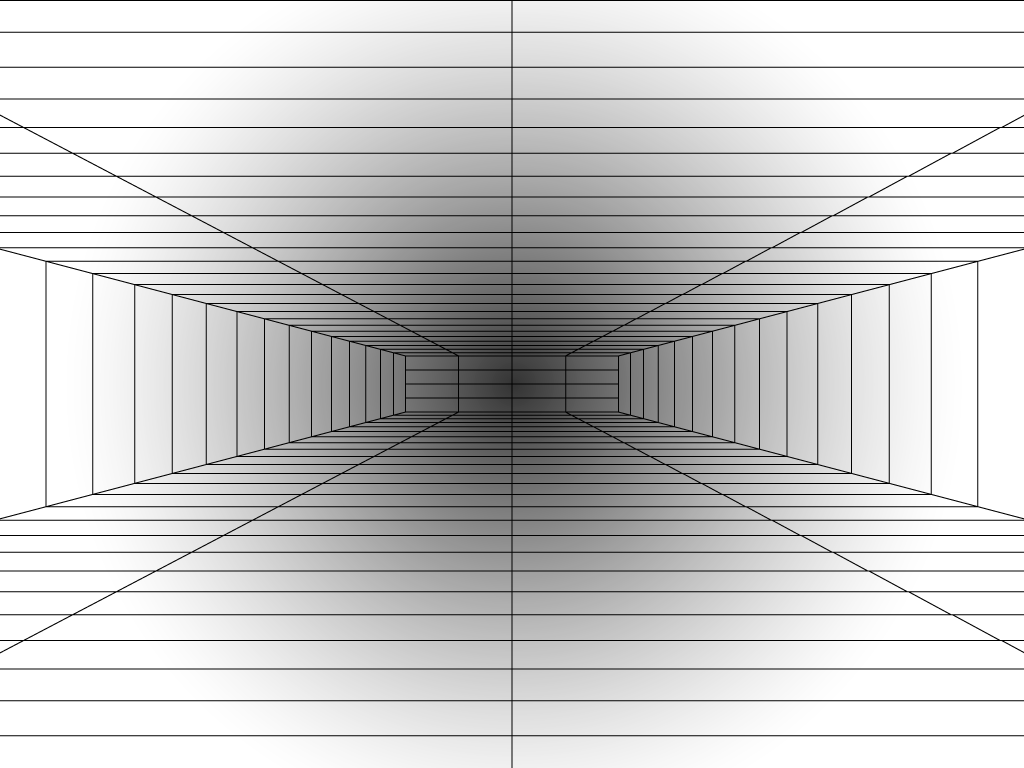
\includegraphics[width=1\linewidth]{figure/Analysis/linearPerspective.png}
	\caption{Linear perspective.}
	\label{fig:linearPerspective}
\end{figure}

\begin{figure}[H]
	\centering
	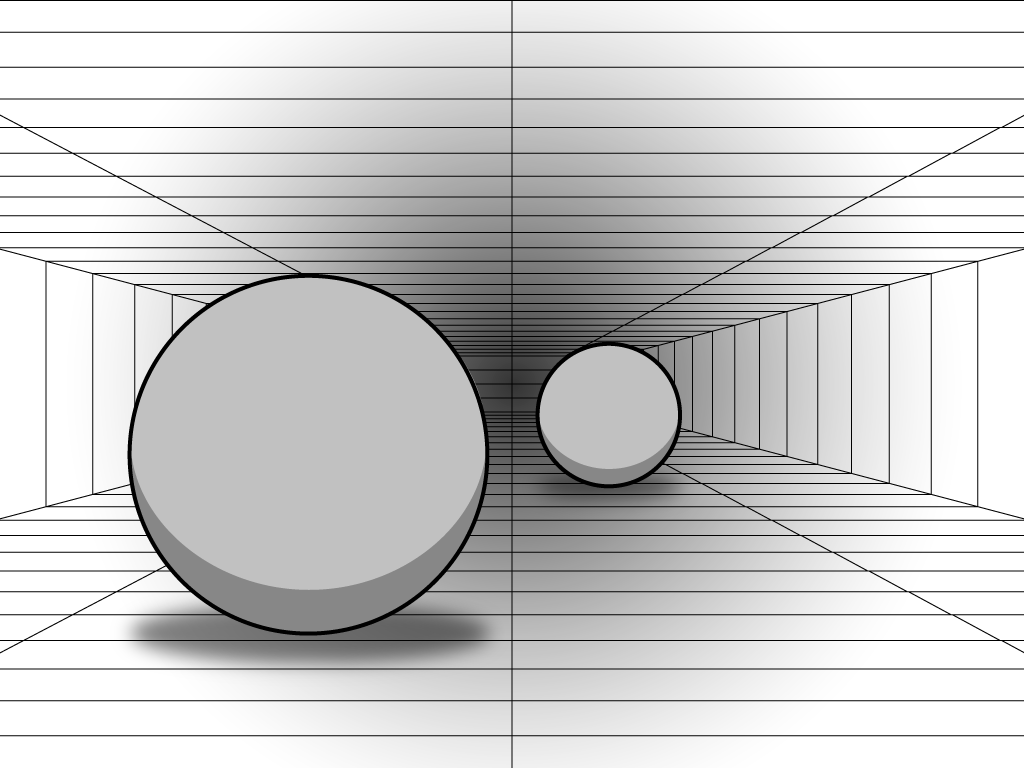
\includegraphics[width=1\linewidth]{figure/Analysis/relativeSize.png}
	\caption{Relative size.}
	\label{fig:relativeSize}
\end{figure}


\begin{figure}[H]
	\centering
	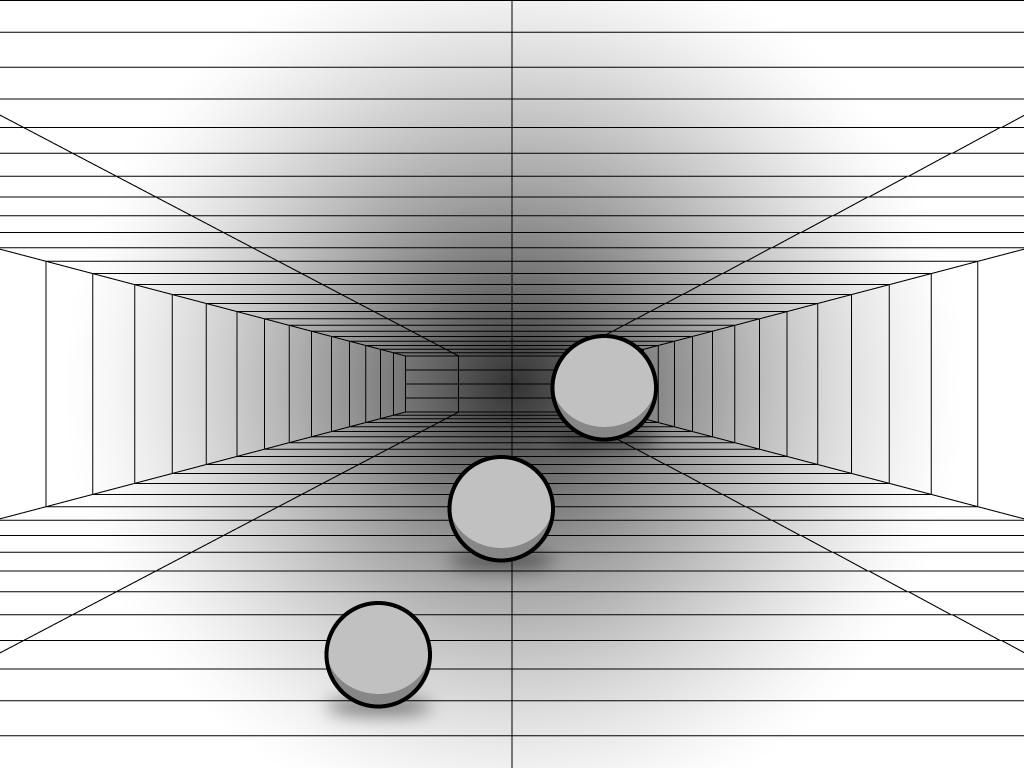
\includegraphics[width=1\linewidth]{figure/Analysis/relativeHeight.png}
	\caption{Relative height.}
	\label{fig:relativeHeight}
\end{figure}


\begin{figure}[H]
	\centering
	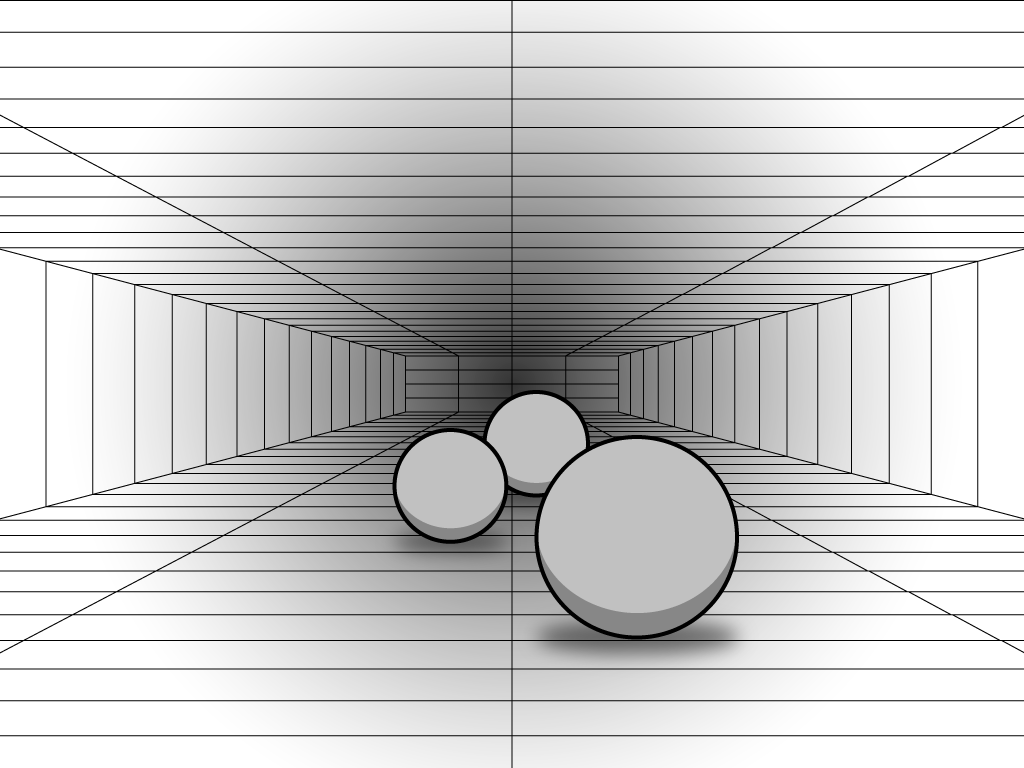
\includegraphics[width=1\linewidth]{figure/Analysis/partialOcclusion.png}
	\caption{Partial occlusion.}
	\label{fig:partialOcclusion}
\end{figure}

\begin{figure}[H]
	\centering
	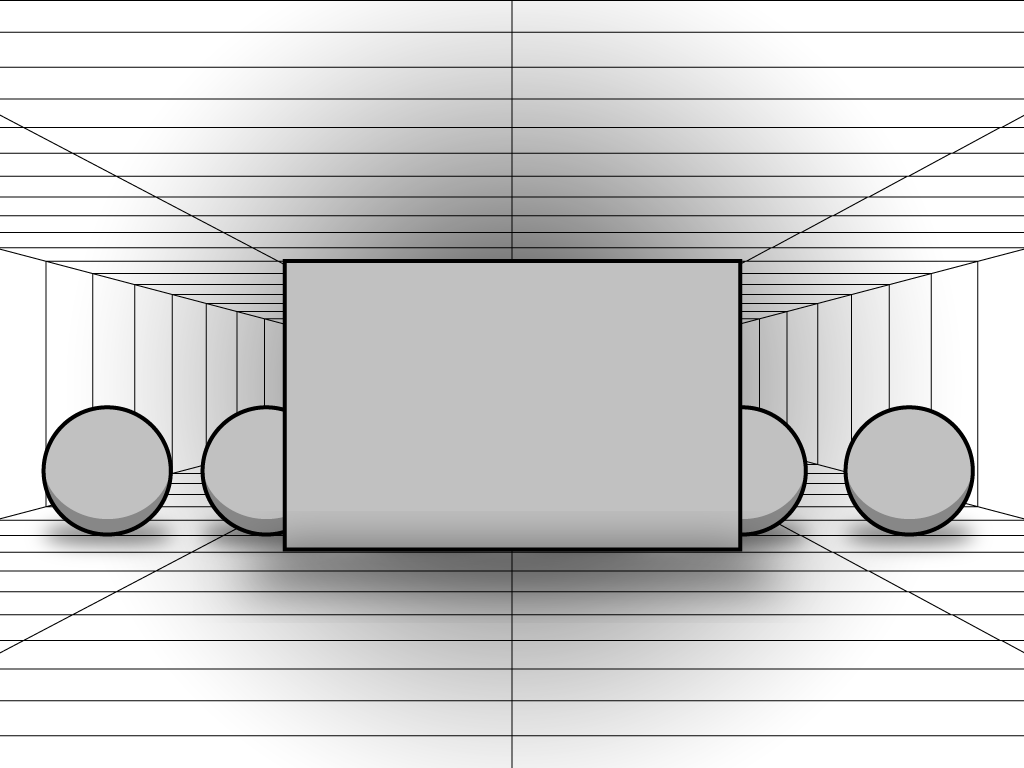
\includegraphics[width=1\linewidth]{figure/Analysis/deletionAccretion.png}
	\caption{Deletion and accretion.}
	\label{fig:deletionAccretion}
\end{figure}

\begin{figure}[H]
	\centering
	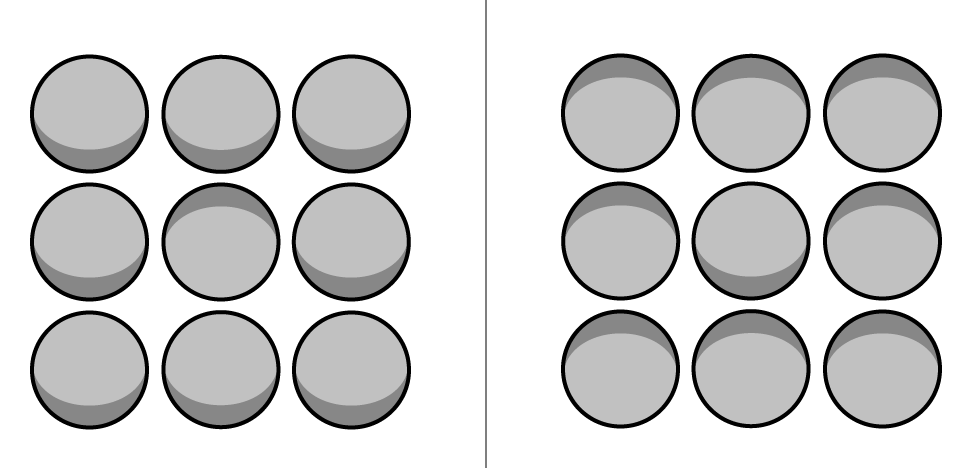
\includegraphics[width=1\linewidth]{figure/Analysis/shading.png}
	\caption{Shading.}
	\label{fig:shading}
\end{figure}

\begin{figure}[H]
	\centering
	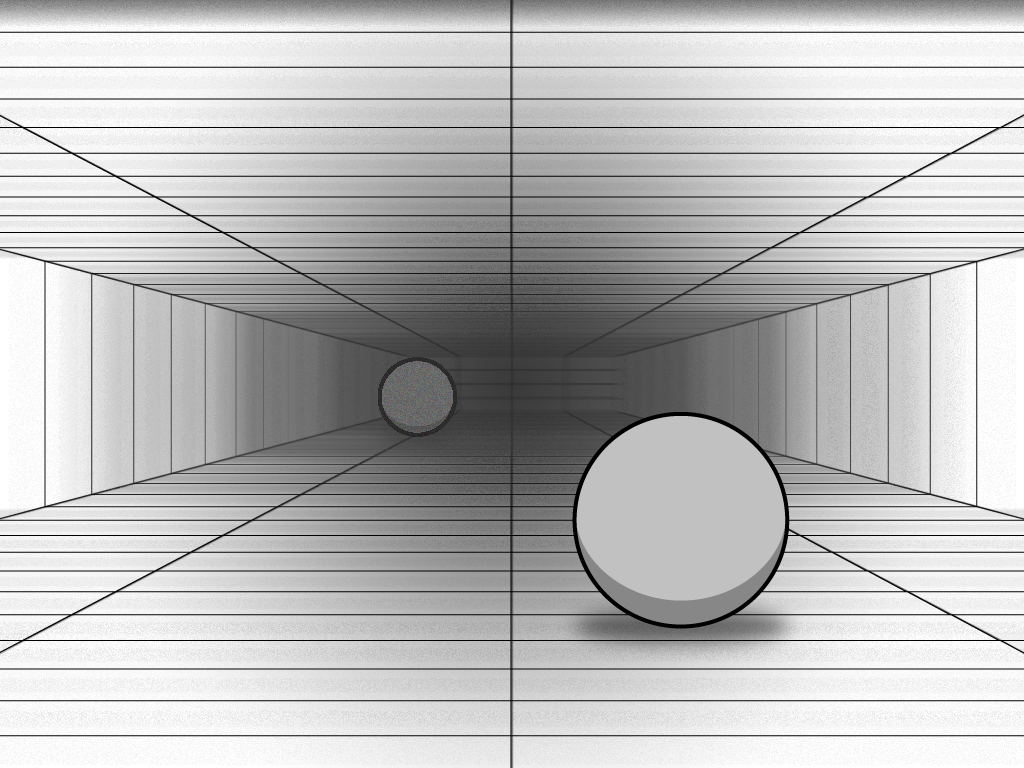
\includegraphics[width=1\linewidth]{figure/Analysis/atmosphericPerspective.png}
	\caption{Atmospheric perspective.}
	\label{fig:atmosphericPerspective}
\end{figure}

\begin{figure}[H]
	\centering
	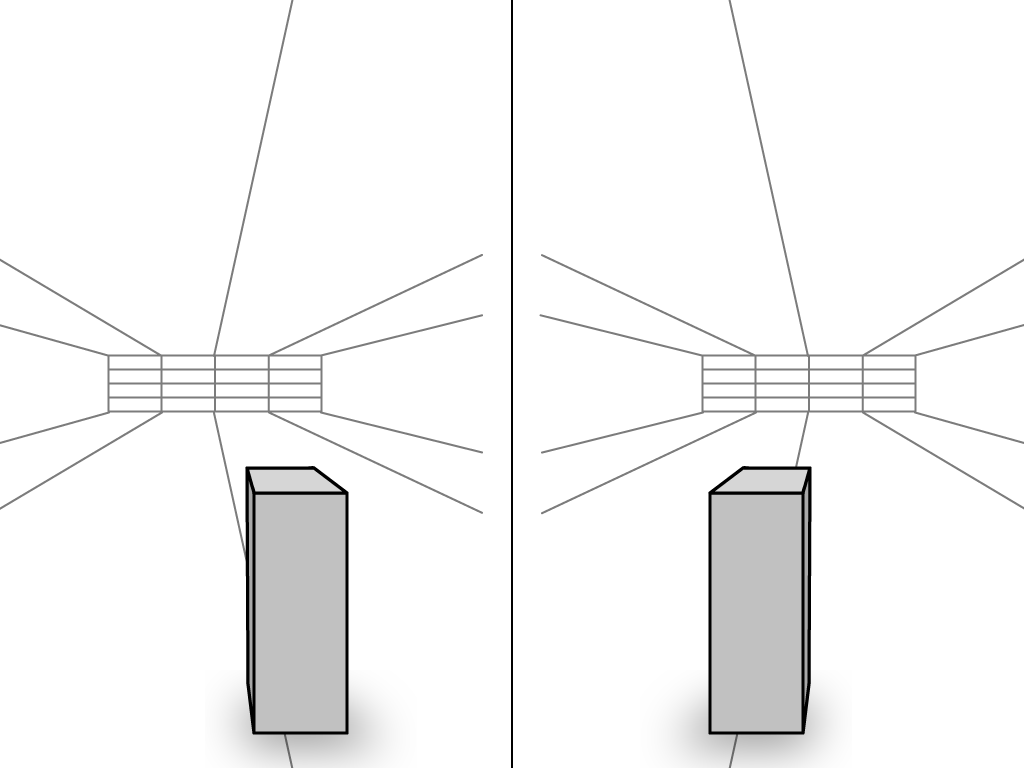
\includegraphics[width=1\linewidth]{figure/Analysis/stereoScopicVision.png}
	\caption{Stereoscopic vision.}
	\label{fig:stereoscopicVision}
\end{figure}
